%%%%%%%%%%%%%%%%%%%%%%%%%%%%%%%%%%%%%%%%%%%%%%%%%%%%%%%%%%%%%%%%%%%%%%%%%%%%%%%%%%%%%%%%%%%%%%%%%%%%%%%%%%%%%%%%%%%%%%%%%%%%%%%%%%%%%%%%%%%%%%%%%%%%%%%%%%%%%%%%%%%
% Written By Michael Brodskiy
% Class: Modern Physics
% Professor: Q. Yan
%%%%%%%%%%%%%%%%%%%%%%%%%%%%%%%%%%%%%%%%%%%%%%%%%%%%%%%%%%%%%%%%%%%%%%%%%%%%%%%%%%%%%%%%%%%%%%%%%%%%%%%%%%%%%%%%%%%%%%%%%%%%%%%%%%%%%%%%%%%%%%%%%%%%%%%%%%%%%%%%%%%

\include{Includes.tex}

\title{The Rutherford-Bohr Model of the Atom}
\date{\today}
\author{Michael Brodskiy\\ \small Professor: Q. Yan}

\begin{document}

\maketitle

\newpage

\tableofcontents

\newpage

\begin{itemize}

    \section{Basic Properties of Atoms}

  \item Around 1900, knowledge about atoms was:

    \begin{itemize}

      \item Size: Small, $1[\si{\angstrom}]/.1[\si{\nano\meter}]$

      \item Stable: Forces balance

      \item Atoms contain electrons ($e^-$) and maintain neutral charge

      \item Atoms can emit and absorb electromagnetic radiation

    \end{itemize}

    \section{Scattering Experiments and the Thomson Model}

  \item An early atom model: J.J. Thomson (1904):

    \begin{figure}[h!]
      \centering
      \tikzset{every picture/.style={line width=0.75pt}} %set default line width to 0.75pt        

\begin{tikzpicture}[x=0.75pt,y=0.75pt,yscale=-1,xscale=1]
%uncomment if require: \path (0,416); %set diagram left start at 0, and has height of 416

%Shape: Circle [id:dp10380104894907105] 
\draw   (172,177) .. controls (172,101.89) and (232.89,41) .. (308,41) .. controls (383.11,41) and (444,101.89) .. (444,177) .. controls (444,252.11) and (383.11,313) .. (308,313) .. controls (232.89,313) and (172,252.11) .. (172,177) -- cycle ;
%Straight Lines [id:da5058547185006379] 
\draw  [dash pattern={on 4.5pt off 4.5pt}]  (308,177) -- (444,177) ;
%Shape: Circle [id:dp045725414249731644] 
\draw   (284,120) .. controls (284,115.58) and (287.58,112) .. (292,112) .. controls (296.42,112) and (300,115.58) .. (300,120) .. controls (300,124.42) and (296.42,128) .. (292,128) .. controls (287.58,128) and (284,124.42) .. (284,120) -- cycle ;
%Shape: Circle [id:dp8094636456513642] 
\draw   (231,186) .. controls (231,181.58) and (234.58,178) .. (239,178) .. controls (243.42,178) and (247,181.58) .. (247,186) .. controls (247,190.42) and (243.42,194) .. (239,194) .. controls (234.58,194) and (231,190.42) .. (231,186) -- cycle ;
%Shape: Circle [id:dp16311007841290293] 
\draw   (336,133) .. controls (336,128.58) and (339.58,125) .. (344,125) .. controls (348.42,125) and (352,128.58) .. (352,133) .. controls (352,137.42) and (348.42,141) .. (344,141) .. controls (339.58,141) and (336,137.42) .. (336,133) -- cycle ;
%Shape: Circle [id:dp3983369960207621] 
\draw   (283,257) .. controls (283,252.58) and (286.58,249) .. (291,249) .. controls (295.42,249) and (299,252.58) .. (299,257) .. controls (299,261.42) and (295.42,265) .. (291,265) .. controls (286.58,265) and (283,261.42) .. (283,257) -- cycle ;
%Shape: Circle [id:dp26761711090461127] 
\draw   (249,149) .. controls (249,144.58) and (252.58,141) .. (257,141) .. controls (261.42,141) and (265,144.58) .. (265,149) .. controls (265,153.42) and (261.42,157) .. (257,157) .. controls (252.58,157) and (249,153.42) .. (249,149) -- cycle ;
%Shape: Circle [id:dp979516059601905] 
\draw   (325,242) .. controls (325,237.58) and (328.58,234) .. (333,234) .. controls (337.42,234) and (341,237.58) .. (341,242) .. controls (341,246.42) and (337.42,250) .. (333,250) .. controls (328.58,250) and (325,246.42) .. (325,242) -- cycle ;

% Text Node
\draw (310,180) node [anchor=north west][inner sep=0.75pt]   [align=left] {$\displaystyle r=.1\left[\text{nm}\right]$};
% Text Node
\draw (292,120) node   [align=left] {\begin{minipage}[lt]{8.67pt}\setlength\topsep{0pt}
\begin{center}
\mbox{-}
\end{center}

\end{minipage}};
% Text Node
\draw (239,186) node   [align=left] {\begin{minipage}[lt]{8.67pt}\setlength\topsep{0pt}
\begin{center}
\mbox{-}
\end{center}

\end{minipage}};
% Text Node
\draw (333,242) node   [align=left] {\begin{minipage}[lt]{8.67pt}\setlength\topsep{0pt}
\begin{center}
\mbox{-}
\end{center}

\end{minipage}};
% Text Node
\draw (344,128) node   [align=left] {\begin{minipage}[lt]{8.68pt}\setlength\topsep{0pt}
\begin{center}
+
\end{center}

\end{minipage}};
% Text Node
\draw (257,144) node   [align=left] {\begin{minipage}[lt]{8.68pt}\setlength\topsep{0pt}
\begin{center}
+
\end{center}

\end{minipage}};
% Text Node
\draw (291,251) node   [align=left] {\begin{minipage}[lt]{8.68pt}\setlength\topsep{0pt}
\begin{center}
+
\end{center}

\end{minipage}};


\end{tikzpicture}

      \caption{The Jelium Model (``Plum-pudding Model'')}
      \label{fig:1}
    \end{figure}

    \section{The Rutherford Nuclear Atom}

  \item Rutherford discovered two rays, $\alpha$ and $\beta$-rays, which he used to experiment with atoms

    \begin{itemize}

      \item $\alpha$ rays are essentially \ce{He^2+} atoms

        \begin{itemize}

          \item The positive charge would mean that the atoms should deflect $\alpha$ rays

        \end{itemize}

    \end{itemize}

  \item The Geiger-Marsden Observation

    \begin{itemize}

      \item Their observation found:

        $$p(\text{backscattering})\approx 10^{-4}$$

      \item This is much larger than expected

      \item Rutherford proposed that the charge and mass of atoms are concentrated in a region called the nucleus

    \end{itemize}

  \item The Bohr Model

    \begin{itemize}

      \item Proposed by Niels Bohr (1913)

      \item Atoms resembled a miniature planetary system

        \begin{figure}[h!]
          \centering
          \tikzset{every picture/.style={line width=0.75pt}} %set default line width to 0.75pt        

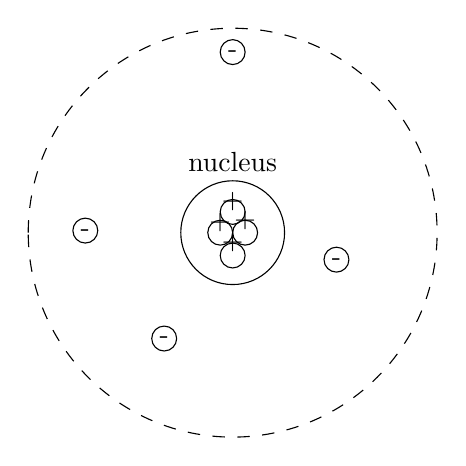
\begin{tikzpicture}[x=0.75pt,y=0.75pt,yscale=-1,xscale=1]
%uncomment if require: \path (0,416); %set diagram left start at 0, and has height of 416

%Shape: Circle [id:dp21437084186170208] 
\draw   (298,185) .. controls (298,171.19) and (309.19,160) .. (323,160) .. controls (336.81,160) and (348,171.19) .. (348,185) .. controls (348,198.81) and (336.81,210) .. (323,210) .. controls (309.19,210) and (298,198.81) .. (298,185) -- cycle ;
%Shape: Circle [id:dp5930049253550815] 
\draw  [dash pattern={on 4.5pt off 4.5pt}] (224.5,185) .. controls (224.5,130.6) and (268.6,86.5) .. (323,86.5) .. controls (377.4,86.5) and (421.5,130.6) .. (421.5,185) .. controls (421.5,239.4) and (377.4,283.5) .. (323,283.5) .. controls (268.6,283.5) and (224.5,239.4) .. (224.5,185) -- cycle ;
%Shape: Circle [id:dp08774721310073264] 
\draw   (317,98) .. controls (317,94.69) and (319.69,92) .. (323,92) .. controls (326.31,92) and (329,94.69) .. (329,98) .. controls (329,101.31) and (326.31,104) .. (323,104) .. controls (319.69,104) and (317,101.31) .. (317,98) -- cycle ;
%Shape: Circle [id:dp561699466772535] 
\draw   (246,184) .. controls (246,180.69) and (248.69,178) .. (252,178) .. controls (255.31,178) and (258,180.69) .. (258,184) .. controls (258,187.31) and (255.31,190) .. (252,190) .. controls (248.69,190) and (246,187.31) .. (246,184) -- cycle ;
%Shape: Circle [id:dp08720949337734774] 
\draw   (367,198) .. controls (367,194.69) and (369.69,192) .. (373,192) .. controls (376.31,192) and (379,194.69) .. (379,198) .. controls (379,201.31) and (376.31,204) .. (373,204) .. controls (369.69,204) and (367,201.31) .. (367,198) -- cycle ;
%Shape: Circle [id:dp44346216911322056] 
\draw   (284,236) .. controls (284,232.69) and (286.69,230) .. (290,230) .. controls (293.31,230) and (296,232.69) .. (296,236) .. controls (296,239.31) and (293.31,242) .. (290,242) .. controls (286.69,242) and (284,239.31) .. (284,236) -- cycle ;
%Shape: Circle [id:dp2819276837978151] 
\draw   (323,185) .. controls (323,181.69) and (325.69,179) .. (329,179) .. controls (332.31,179) and (335,181.69) .. (335,185) .. controls (335,188.31) and (332.31,191) .. (329,191) .. controls (325.69,191) and (323,188.31) .. (323,185) -- cycle ;
%Shape: Circle [id:dp9065404250880571] 
\draw   (311,185) .. controls (311,181.69) and (313.69,179) .. (317,179) .. controls (320.31,179) and (323,181.69) .. (323,185) .. controls (323,188.31) and (320.31,191) .. (317,191) .. controls (313.69,191) and (311,188.31) .. (311,185) -- cycle ;
%Shape: Circle [id:dp744122974738064] 
\draw   (317,175) .. controls (317,171.69) and (319.69,169) .. (323,169) .. controls (326.31,169) and (329,171.69) .. (329,175) .. controls (329,178.31) and (326.31,181) .. (323,181) .. controls (319.69,181) and (317,178.31) .. (317,175) -- cycle ;
%Shape: Circle [id:dp46454223972535336] 
\draw   (317,196) .. controls (317,192.69) and (319.69,190) .. (323,190) .. controls (326.31,190) and (329,192.69) .. (329,196) .. controls (329,199.31) and (326.31,202) .. (323,202) .. controls (319.69,202) and (317,199.31) .. (317,196) -- cycle ;

% Text Node
\draw (323,157) node [anchor=south] [inner sep=0.75pt]   [align=left] {nucleus};
% Text Node
\draw (323,98) node   [align=left] {\begin{minipage}[lt]{8.67pt}\setlength\topsep{0pt}
\begin{center}
\mbox{-}
\end{center}

\end{minipage}};
% Text Node
\draw (373,198) node   [align=left] {\begin{minipage}[lt]{8.67pt}\setlength\topsep{0pt}
\begin{center}
\mbox{-}
\end{center}

\end{minipage}};
% Text Node
\draw (290,236) node   [align=left] {\begin{minipage}[lt]{8.67pt}\setlength\topsep{0pt}
\begin{center}
\mbox{-}
\end{center}

\end{minipage}};
% Text Node
\draw (252,184) node   [align=left] {\begin{minipage}[lt]{8.67pt}\setlength\topsep{0pt}
\begin{center}
\mbox{-}
\end{center}

\end{minipage}};
% Text Node
\draw (329,179) node   [align=left] {\begin{minipage}[lt]{8.68pt}\setlength\topsep{0pt}
\begin{center}
+
\end{center}

\end{minipage}};
% Text Node
\draw (323,190) node   [align=left] {\begin{minipage}[lt]{8.68pt}\setlength\topsep{0pt}
\begin{center}
+
\end{center}

\end{minipage}};
% Text Node
\draw (317,180) node   [align=left] {\begin{minipage}[lt]{8.68pt}\setlength\topsep{0pt}
\begin{center}
+
\end{center}

\end{minipage}};
% Text Node
\draw (323,170) node   [align=left] {\begin{minipage}[lt]{8.68pt}\setlength\topsep{0pt}
\begin{center}
+
\end{center}

\end{minipage}};


\end{tikzpicture}

          \caption{The Bohr Model}
          \label{fig:2}
        \end{figure}

      \item From this, the Coulomb interaction (force) was determined:

        $$\boxed{F=\frac{1}{4\pi\varepsilon_o}\frac{|q_1||q_2|}{r^2}}$$

      \item The kinetic energy was determined as:

        $$\boxed{K=\frac{1}{8\pi\varepsilon_o}\frac{e^2}{r}}$$

      \item If the electron is radiating, it slows down and moves toward nucleus to collapse?

        \begin{itemize}

          \item Niels Bohr hypothesized that electrons may exist in ``stationary states'' without radiating electromagnetic energy

        \end{itemize}

      \item $L = rp = rmv = n\hbar \rightarrow v = \frac{n\hbar}{mr}$

        \begin{itemize}

          \item Where $L$ is the angular momentum, $r$ is the radius, n is a quantized number, and $m$ is the mass

        \end{itemize}

      \item Substituting this into kinetic energy, we get the permitted radius, $r$:

        $$\boxed{r_n=\frac{4\pi\varepsilon_o\hbar^2}{me^2}n^2}$$

      \item Using electron information, we get:

        $$\frac{4\pi\varepsilon_o\hbar^2}{me^2}=.0529[\si{\nano\meter}]$$

      \item This value is known as the Bohr radius

    \end{itemize}

  \item Hydrogen Atom and Bohr Model:

    \begin{itemize}

      \item Radius: $r_n=a_on^2,\quad\quad n=1,2,3$

      \item Energy: $E_n=\frac{-13.6[\si{\eV}]}{n^2}$

      \item $\Delta E = E_n - E_1$ is the excitation energy, where $E_n$ is the nth excited state, and $E_1$ is the ground state

        \begin{itemize}

          \item $|E_n|$ is the binding energy of $e^-$ in state $n$ (ionization energy)

        \end{itemize}

      \item Optical transitions\footnote{Transitions using a photon}  result in absorption or emission of a photon

        \begin{itemize}

          \item In stationary state, there is no electromagnetic energy radiation

          \item $e^-$ can emit radiation when moving from $n_1$ to $n_2$

        \end{itemize}

    \end{itemize}

    \section{Line Spectra}

  \item The absorption or emission from atoms may be used to create an emission spectra

  \item A general equation was generated:

    $$\boxed{\lambda=\lambda_{\text{limit}}\dfrac{n^2}{n^2-n_o^2},\quad\quad n=n_o+1,n_o+2,\cdots}$$

  \item For the Balmer series, $n_o=2$

  \item For the Lyman series, $n_o=1$
    
  \item The Ritz combination principle:

    $$f_1+f_2=f_3$$

    \begin{itemize}

      \item This principle shows that the sum of any two emission frequencies results in a frequency that is also in the spectrum

    \end{itemize}

  \item The wavelength of the transition becomes:

    $$\lambda=\frac{c}{f}=\dfrac{64\pi^3\varepsilon_o^2\hbar^3c}{me^4}\dfrac{n_1^2n_2^2}{n_1^2-n_2^2}=\dfrac{1}{R_{\infty}}\dfrac{n_1^2n_2^2}{n_1^2-n_2^2}$$

  \item Where $R_{\infty}$ is the Rydberg constant, equal to $1.097\cdot10^7 [\si{\per\meter}]$

  \item Lyman series are only observed in the absorption spectrum

  \item The following summarizes emission spectra

    \begin{itemize}

      \item Isolated atoms are in the ground state most of the time

      \item Excited state lives fro a short time (picoseconds to femtoseconds)

      \item The absorption spectrum only occurs from the ground state

      \item Balmer series are not found in the absorption spectrum

    \end{itemize}

    \section{The Bohr Model}

  \item For an atom with $z>1$

    \begin{itemize}

      \item For a nucleus of charge $ze$, the Coulomb force is:

        $$F=\frac{1}{4\pi\varepsilon_o}\frac{|q_1||q_2|}{r^2}=\frac{ze^2}{4\pi\varepsilon_o r^2}$$

    \end{itemize}

\end{itemize}

\end{document}

